
\documentclass[12pt]{article}
\usepackage[a4paper, margin=.30in]{geometry}
\usepackage{graphicx ,
            wrapfig,
            xcolor, 
            enumerate,
            amsmath,
			fontenc,
			tcolorbox,circuitikz,tikz,bm
            }
			\usepackage{pgfplots}
\pgfplotsset{compat=newest}
\usepgfplotslibrary{fillbetween}
\usepackage{pgfplots}
\newcommand\headerMe[2]{\noindent{}#1\hfill#2}
\renewcommand{\thesection}{\Roman{section}}

\author{Zakaria HAOUZAN}
\date{\today}

\begin{document}
% headers --------------
\headerMe{Matière : Physique-Chimie}{Professeur : Zakaria HAOUZAN}\\
\headerMe{Unité : Mécanique }{Établissement : Lycée SKHOR qualifiant}\\
\headerMe{Niveau : 2BAC-SM-PC}{Heure : 6H}\\

% ------Content ________
\begin{center}

    \Large{Leçon $N^{\circ} 15 $: \color{red}Systèmes oscillants.}
\end{center}


\section{Les Systèmes mécaniques oscillants.}


\begin{wrapfigure}[1]{r}{0.2\textwidth} 
	\vspace{-4cm}
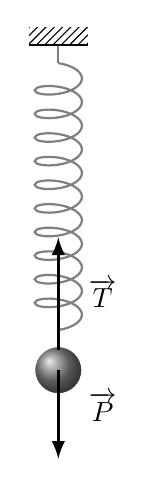
\begin{tikzpicture} [scale=0.75, decoration={coil,aspect=0.4,segment length=3mm,amplitude=3mm}]
%decoration : gère l'aspect du ressort par l'instruction decorate
\tikzset{ressort/.style={thick,gray,smooth}} %définition d'un style de ressort
\usetikzlibrary{patterns}
\begin{scope}[xshift=6cm]
\draw[ressort,decorate] (0,-0.3)--(0,-5) ;

%bloc qui tient le ressort
\draw[thick,gray] (0,0) -- (0,-0.3); \fill [pattern=north east lines] (-0.5,0) rectangle (0.5,0.3);
%pattern définit un style de remplissage de la forme
\draw[thick](-0.5,0)--(0.5,0); %fin ressort

\draw [thick](0,-5)--(0,-5.5);
\draw [rounded corners=4pt,color=white,ball color=gray,smooth] (0,-5.5) circle (0.4) ;

\draw [very thick,-latex] (0,-5.5)--++(0,-1.5) node [midway,above=0.1cm,right=0.25cm] {$\overrightarrow{P}$};
\draw [very thick,-latex] (0,-5.15)--(0,-3.25) node [midway,right=0.25cm] {$\overrightarrow{T}$};
\end{scope}
\end{tikzpicture}


%--------------------- Pendule et base polaire -----------

	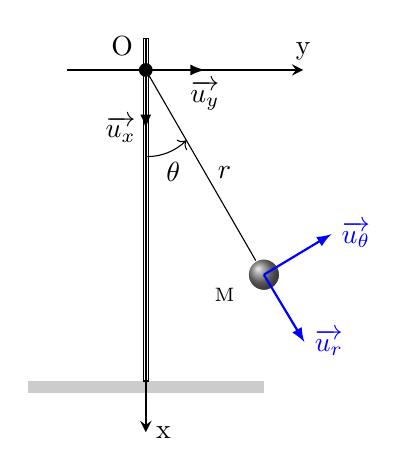
\begin{tikzpicture}[scale=1] 
% \node[,inner sep=0] at (0.75,4.05) {\includegraphics[scale=0.2]{capitaine.pdf}}; 
	\fill [gray,opacity=0.4] (0,-0.5) rectangle (3,-0.35);
	\draw (1.47,-0.35) rectangle (1.53,4);
	% \filldraw [gray,opacity=0.4] (1,3.5) arc (-180:0:0.5);
	% \draw [gray]  (1,3.5) -- (2,3.5);      
	
	\draw [->] (1.52,2.5) arc (-90:-45:0.7); 
	\node at (1.85,2.3) {$\theta$}; 
	
	
	%repère cartésien                                               
	\node at (1.2,3.9) {O};
	\draw [->,-stealth,thick] (0.5,3.6) --++ (3,0) node [above] {y};
	\draw [->,-latex,thick] (1.5,3.6) --++ (0.75,0) node [below] {$\overrightarrow{u_y}$};
	\draw [->,-stealth,thick] (1.5,4) --++ (0,-5) node [right] {x};
	\draw [->,-latex,thick] (1.5,3.6) --++ (0,-0.75) node [left] {$\overrightarrow{u_x}$};		              
	%fin

	\draw node at (2.5,2.3) {$r$}; 

	\filldraw [black] (1.5,3.6) circle (0.08cm);
	\draw [black] (1.5,3.6) -- (3,1);
	\draw [color=white,ball color=gray,smooth] (3,1) circle (0.2); 
	\node at (2.5,0.75) {\scriptsize{M}} ;
	% \draw [blue,->,-latex] (3,1) -- (3,0.2) node [left] {$\overrightarrow{P}$};
	% \draw [red,->,-latex] (2.9,1.17) -- (2.48,1.9) node [right] {$\overrightarrow{T}$};    
 
	 \draw [-latex, thick, blue] (3,1) --++ (-59:1) node [right] {$\overrightarrow{u_r}$};  
	
	 \draw [-latex,thick,blue] (3,1) --++ (31:1) node [right] {$\overrightarrow{u_{\theta}}$};   
	
	% \draw [dashed] (3,1)--++(0,2.6);                                               
	% \draw [dashed] (3,1)--++(-1.5,0); 
	\label{pendule_base_polaire}	                                              
	\end{tikzpicture}


%%--------------------- Pendule et base polaire -----------

	%\begin{tikzpicture}[scale=1] 
	%\fill [gray,opacity=0.4] (0,-0.5) rectangle (3,-0.35);
	%\draw (1.47,-0.35) rectangle (1.53,4);
	
	%\draw [->] (1.52,2.5) arc (-90:-45:0.7); 
	%\node at (1.85,2.3) {$\theta$}; 
	
	
	%%repère cartésien                                               
	%\node at (1.2,3.9) {O};
	%\draw [->,-stealth,thick] (0.5,3.6) --++ (3,0) node [above] {y};
	%\draw [->,-latex,thick] (1.5,3.6) --++ (0.75,0) node [below] {$\overrightarrow{u_y}$};
	%\draw [->,-stealth,thick] (1.5,4) --++ (0,-5) node [right] {x};
	%\draw [->,-latex,thick] (1.5,3.6) --++ (0,-0.75) node [left] {$\overrightarrow{u_x}$};		              
	%%fin

	%\draw node at (2.5,2.3) {$L$}; 

	%%\filldraw [black] (1.5,3.6) circle (0.08cm);
	%\draw [black ,line width=0.1cm] (1.5,3.6) -- (3,1);
	%%\draw [color=white,ball color=gray,smooth] (3,1) circle (0.2); 
	%\node at (2.5,0.75) {\scriptsize{M}} ;
 
	
	
	 %\draw [dashed] (3,1)--++(0,2.6);                                               
	 %\draw [dashed] (3,1)--++(-1.5,0); 
	%\label{pendule_base_polaire}	                                              
	%\end{tikzpicture}

\end{wrapfigure}




\subsection{Exemples de quelques oscillateurs mécaniques:}
On donne quelques exemples de systèmes mécaniques oscillants:

\begin{itemize}

	\item \textbf{\underline{Le pendule élastique}} : il est constitué d'un corps solide de masse m \\suspendu à un resort à spires non jointives.

	\item \textbf{\underline{Le pendule simple}} : il est constitué d'un corps solide de masse m suspendu \\à l'extremité d'un fil inextensible.
	\item  \textbf{\underline{Le pendule pesant:}} est tout corps solide mobile autour d'un axe ne passant pas\\ par son centre de gravité
	\item \textbf{\underline{Le pendule de torsion}}: est constitué d'une barre horizontale, fixée à l'extremité d'un \\fil de torsion.

\end{itemize}

D'une façon générale un oscillateur mécanique , effectue des oscillations autour de sa position d'équilibre .

\subsection{Caractéristiques des mouvements oscillatoires: }
Un mouvement oscillatoire est caractérisé par:
\begin{itemize}
	\item \textbf{Sa position d'équilibre }  stable c'est la position à laquelle le système tend à y revenir lorsque l'on en éloigne légèrement.
\item \textbf{Sa période propre} : c'est le temps mis pour effectuer une oscillation.
\item  \textbf{Son amplitude} : c'est la valeur maximale positive que prend la grandeur qui exprime le décalage ou l'inclinaison de l'oscillateur
de sa position d'équilibre.

\end{itemize}

\begin{center}
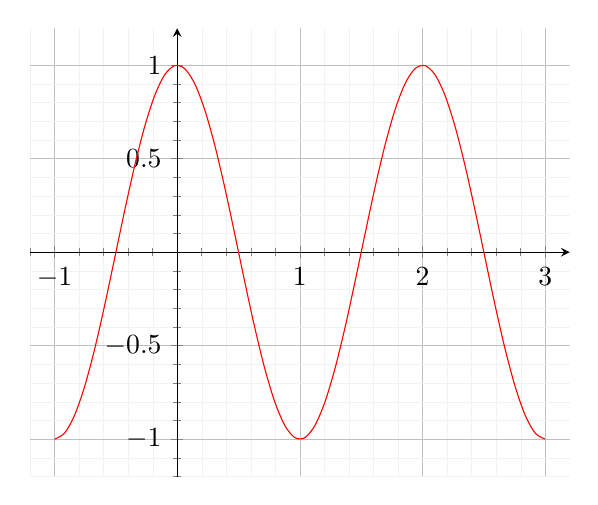
\begin{tikzpicture}
  \begin{axis}%
    [grid=both,
     minor tick num=4,
     grid style={line width=.1pt, draw=gray!10},
     major grid style={line width=.2pt,draw=gray!50},
     axis lines=middle,
     enlargelimits={abs=0.2}
    ]
    \addplot[domain=-1:3,samples=50,smooth,red] {cos(deg(pi*x))};
  \end{axis}
\end{tikzpicture}
\end{center}
\subsection{Amortissement des oscillations: }

\subsubsection{Définition:}

En écartant un pendule élastique de sa position d'équilibre et en le lâchant, l'amplitude des oscillations diminue jusqu'à ce qu'il
s'annule: on dit que le mouvement est amorti. Le phénomène d'amortissement est provoqué par les frottements.
Il existe deux types de frottements :
\begin{itemize}
	\item Le frottement solide qui se fait entre l'oscillateur et un corps solide.
	\item Le frottement fluide qui se fait entre l'oscillateur et un corps fluide (liquide ou gaz) .
\end{itemize}

\subsubsection{Les régimes d'amortissement: }

\textbf{Le régime pseudo périodique }:si l'amortissement est faible, l'amplitude des oscillations diminue progressivement
jusqu'à ce qu'il s'annule.



\begin{center}

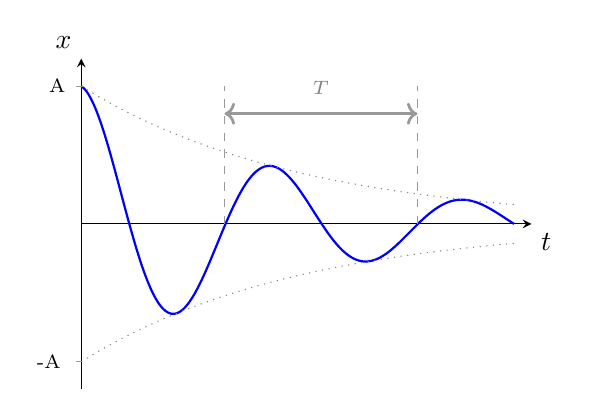
\begin{tikzpicture}[scale=0.7]
%papier milli
%\draw [very thin, gray!10] (0,-3) grid[step=0.1] (2.5*pi,3);
%\draw [very thin, black!10] (0,-3) grid[step=0.5] (2.5*pi,3);
%\draw [very thin, black!20] (0,-3) grid[step=1] (2.5*pi,3);
%fin

%axes
\draw[->,>=stealth] (0,0) -- (2.6*pi,0) node[below right] {$t$};
\draw[->,>=stealth] (0,-3) -- (0,3) node [above left] {$x$};
%\draw (1,0.1) -- (1,-0.1) node [below right] {{\scriptsize $0.2$}}; %échelle abscisse
%\draw (0.1,1) -- (-0.1,1) node [left] {{\scriptsize $2V$}}; %échelle ordonnée
%fin

%legende
%\draw (-2,3) -- (-0.4,3) -- (-0.4,1.9) -- (-2,1.9) -- (-2,3); %cadre
%\draw [red] (-1.8,2.7)--(-1.2,2.7) node [right] [red] {$V_E$};
%\draw [blue] (-1.8,2.2)--(-1.2,2.2) node [right] [blue] {$V_S$};
%fin

%Courbe principale
\draw[color=blue,thick,domain=0:2.5*pi, samples=150,smooth] plot ({\x},{2.5*exp(-\x/4)*sin(1.8*\x r + pi/2 r)});

%enveloppe 
\draw[color=gray,thin,dotted,domain=0:2.5*pi, samples=150,smooth] plot ({\x},{2.5*exp(-\x/4)});
\draw[color=gray,thin,dotted,domain=0:2.5*pi, samples=150,smooth] plot ({\x},{-2.5*exp(-\x/4)});
%double flèche
\draw[gray!80,line width=1pt,<->] (2.6,2) --++ (3.5,0) node [midway, above] {\colorbox{white}{\textcolor{gray}{\scriptsize{$T$}}}} ;
%Fin
%pointillés
\draw [very thin,gray!80, dashed] (2.6,0) --++ (0,2.5);
\draw [very thin,gray!80, dashed] (6.1,0) --++ (0,2.5);
\draw [very thin,gray!80, dashed] (-0.1,2.5) --++ (0.2,0) node [left=0.15cm, black] {\scriptsize{A}};
\draw [very thin,gray!80, dashed] (0,-2.5) --++ (-0.1,0) node [left=0.07cm, black] {\scriptsize{-A}};
\end{tikzpicture}


\end{center}





\textbf{Le régime apériodique} : si le frottement est fort les oscillations disparaissent et selon l'importance de l'amortissement on
distingue trois régimes:

\begin{itemize}

	\item Le régime sous critique : l'oscillateur effectue une seule oscillation avant de s'arrêter.
	\item Le régime critique : l'oscillateur revient à sa position d'équilibre sans oscillations.
	\item Le régime surcritique l'oscillateur revient à sa position d'équilibre après temps très long sans oscillations.

\end{itemize}

\begin{center}


	   %%------------------- Régimes apériodiques -------------


%\begin{tikzpicture}[scale=1]
%% \def \lbd{2}
%\def \ome{1.8}
%% \def \rmoins{(-\lbd-(\lbd^2-\ome^2)^0.5)}
%% \def \rplus{(-\lbd+(\lbd^2-\ome^2)^0.5)}

%%papier milli
%%\draw [very thin, gray!10] (0,-3) grid[step=0.1] (2.5*pi,3);
%%\draw [very thin, black!10] (0,-3) grid[step=0.5] (2.5*pi,3);
%%\draw [very thin, black!20] (0,-3) grid[step=1] (2.5*pi,3);
%%fin

%%axes
%\draw[->,>=stealth] (0,0) -- (2.6*pi,0) node[below right] {$t$};
%\draw[->,>=stealth] (0,-1) -- (0,3) node [above left] {$x$};
%%\draw (1,0.1) -- (1,-0.1) node [below right] {{\scriptsize $0.2$}}; %échelle abscisse
%%\draw (0.1,1) -- (-0.1,1) node [left] {{\scriptsize $2V$}}; %échelle ordonnée
%%fin

%%legende
%%\draw (-2,3) -- (-0.4,3) -- (-0.4,1.9) -- (-2,1.9) -- (-2,3); %cadre
%%\draw [red] (-1.8,2.7)--(-1.2,2.7) node [right] [red] {$V_E$};
%%\draw [blue] (-1.8,2.2)--(-1.2,2.2) node [right] [blue] {$V_S$};
%%fin
%\foreach \lbd/\color in {2/blue, 3/orange, 4/red}
%{   
 %\def \rmoins{(-\lbd-(\lbd^2-\ome^2)^0.5)}
%\def \rplus{(-\lbd+(\lbd^2-\ome^2)^0.5)}

%\draw[color=\color,thick,domain=0:2.5*pi, samples=150,smooth] plot ({\x},{((2.5*\rmoins)*exp(\rplus*\x))/(\rmoins-\rplus)-((2.5*\rplus)*exp(\rmoins*\x)/(\rmoins-\rplus)});  
%}     
%\draw (3.75,1.75) rectangle++ (2.5,1.5);
%\draw [blue] (4,3) --++ (0.5,0) node [shift=({0.75,0})] {: $\lambda = 2$};
%\draw [orange] (4,2.5) --++ (0.5,0) node [shift=({0.75,0})] {: $\lambda = 3$};
%\draw [red] (4,2) --++ (0.5,0) node [shift=({0.75,0})] {: $\lambda = 4$};

%%pointillés

%\draw [very thin,gray!80, dashed] (-0.1,2.5) --++ (0.2,0) node [left=0.15cm, black] {\scriptsize $x_m$};

%\end{tikzpicture}




\end{center}

\section{Etude de quelques systèmes mécanique oscillants}
\subsection{Le pendule Élastique horizontale  : }



Il est constitué d'un ressort posé sur un banc à coussin d'air horizontal comme l'indique la figure suivante:

\begin{center}
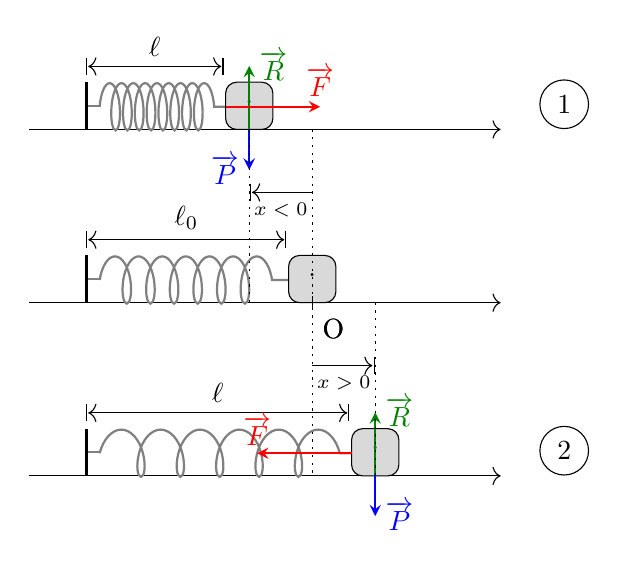
\begin{tikzpicture}[scale=0.8]
	
\tikzset{ressort/.style={thick,gray,smooth}} %définition d'un style de ressort
	\usetikzlibrary{patterns}
\coordinate (O) at (0,-2.75); 
	\draw [->] (-4.5,-2.75) -- (3,-2.75) ;
\begin{scope}[shift=({0,-2.75})]     

	\begin{scope}[scale=0.75,shift=({-4.78,0.5}),rotate around={90:(0,0)}]
	  %bloc qui tient le ressort

		\draw[thick,gray] (0,0) -- (0,-0.3); 
		%\fill [pattern=north east lines] (-0.5,0) rectangle (0.5,0.3); 
		\draw[thick](-0.5,0)--(0.5,0);
		%fin ressort       
	\end{scope}
	 \draw [ressort,decorate,decoration={coil,aspect=0.4,segment length=3mm,amplitude=3mm}] (-3.375,0.36)--++(3,0) ;
	 \draw[rounded corners=4pt,fill=gray!30] (-0.375,0) rectangle++ (0.75,0.75) node [midway, shift=({0,0.05})] {$.$};  
 %repérage de \ell
	\draw [|<->|] (-3.6,1) -- (-0.4,1) node [midway,above] {$\ell_0$}; 
\end{scope}

%--------------------FIN ressort central---------------------	


	%----------ressort comprimé------------
	\coordinate (M) at (-1,0.36);
	\draw (O) --++ (0,0.1) (O) --++ (0,-0.1) node [below right] {O}; 
    
	\node[draw, circle] at (4,0.4) {1};  

	%Axe
	\draw [->] (-4.5,0) -- (3,0) ;  

	%repérage de x
	\draw [|<-] (-1,-1) -- (0,-1) node [midway,below] {\scriptsize  $x<0$};

	%repérage de \ell
	\draw [|<->|] (-3.6,1) -- (-1.4,1) node [midway,above] {$\ell$};

	\begin{scope}[scale=0.75,shift=({-4.78,0.5}),rotate around={90:(0,0)}]
	  %bloc qui tient le ressort
		\draw[thick,gray] (0,0) -- (0,-0.3); 
		\draw[thick](-0.5,0)--(0.5,0);
		%fin ressort       
	\end{scope}	   

	%ressort  
	\draw [ressort,decorate,decoration={coil,aspect=0.3,segment length=1.5mm,amplitude=3mm}] (-3.375,0.36)--++(2,0) ;
	\draw[rounded corners=4pt,fill=gray!30] (-1.375,0) rectangle++ (0.75,0.75) node [midway, shift=({0,0.05})] {$.$}; 

	\draw [->,-stealth,thick,blue] (M) --++(0,-1) node [left] {$\overrightarrow{P}$};   
	\draw [->,-stealth,thick,green!50!black] (M)++(0,-0.35) --++(0,+1) node [right] {$\overrightarrow{R}$};   
	\draw [->,-stealth,thick,red] (M)++(-0.375,0)--++(1.5,0) node [above] {$\overrightarrow{F}$};     
	%----------FIN ressort comprimé------------ 

%----------ressort etiré------------

	\begin{scope}[shift=({0,-5.5})]

	\coordinate (M) at (1,0.36);
	\draw (O) --++ (0,0.1) (O) --++ (0,-0.1) node [below right] {O}; 
     
	\node[draw, circle] at (4,0.4) {2};
   

	%Axe
	\draw [->] (-4.5,0) -- (3,0) ;  

	%repérage de x
	\draw [->|] (0,1.75) -- (1,1.75) node [midway,below] {\scriptsize $x>0$};

	%repérage de \ell
	\draw [|<->|] (-3.6,1) -- (0.6,1) node [midway,above] {$\ell$};

	\begin{scope}[scale=0.75,shift=({-4.78,0.5}),rotate around={90:(0,0)}]
	  %bloc qui tient le ressort
		\draw[thick,gray] (0,0) -- (0,-0.3); 
		\draw[thick](-0.5,0)--(0.5,0);
		%fin ressort       
	\end{scope}	   

	%ressort  
	\draw [ressort,decorate,decoration={coil,aspect=0.5,segment length=5mm,amplitude=3mm}] (-3.375,0.36)--++(4,0) ; 

	 \draw[rounded corners=4pt,fill=gray!30] (0.625,0) rectangle++ (0.75,0.75) node [midway, shift=({0,0.05})] {$.$}; 

	\draw [->,-stealth,thick,blue] (M) --++(0,-1) node [right] {$\overrightarrow{P}$};   
	\draw [->,-stealth,thick,green!50!black] (M)++(0,-0.35) --++(0,+1) node [right] {$\overrightarrow{R}$};   
	\draw [->,-stealth,thick,red] (M)++(-0.375,0)--++(-1.5,0) node [above=-1] {$\overrightarrow{F}$};	


	\end{scope}    

	\draw [dotted] (-1,0) --++(0,-2.75);  
	\draw [dotted] (1,-2.75) --++(0,-2.75);  
	\draw [dotted] (0,0) --++(0,-5.5);  

\end{tikzpicture}
\end{center}

Après avoir mis en marche la soufflerie, on écarte la cavalier horizontalement d'une distance xm puis on le lâche , il effectue
des oscillations non amorties.

\textbf{Equation différentielle du mouvement: }
\begin{itemize}
	\item Le système étudié {le cavalier}

	\item Bilan des forces : Le cavalier lors de son mouvement oscillatoire est soumis à l'action des forces suivantes:
		\begin{itemize}
			\item $\vec{P}$ : son poids.
			\item $\vec{R}$ :la réaction du banc à coussin d'air ( elle est perpendiculaire au plan de contact car les frottements sont négligeables).
			\item $\vec{T}$ : la tension du ressort , c’est une force de rappel $\vec{T} = -T\vec{i}$.
(Elle s’oppose toujours à l’allongement du ressort et elle est proportionnelle à cet allongement).
		\end{itemize}
	\item Application de la deuxième loi de Newton : $\sum \vec{F_{ext}} = m.\vec{a_G}$

		par projection sur l'axe Ox : $m.\ddot{x} + K.x = 0$

		d’où: $\ddot{x} + \frac{K}{m}.x = 0$ C'est l'équation différentielle du mouvement

\end{itemize}

\textbf{Solution de l'équation différentielle du mouvement : }

La solution de l'équation différentielle du mouvement $\ddot{x} + \frac{K}{m}.x = 0$
est une fonction sinusoidale qui s'écrit sous la forme suivante: $$x(t) = x_m.cos(\omega_0.t + \phi)$$

\begin{center}
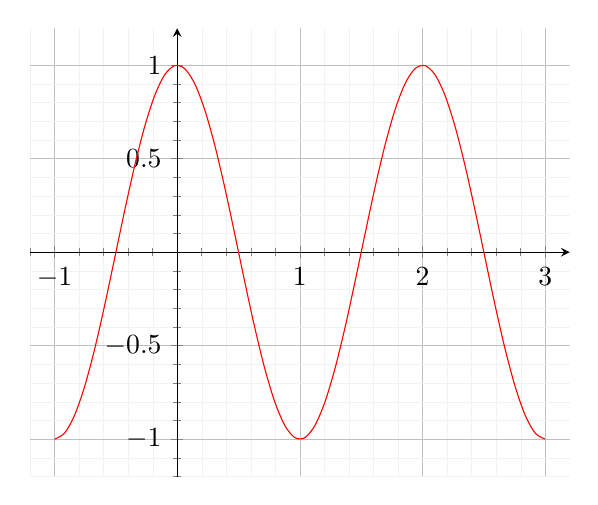
\begin{tikzpicture}
  \begin{axis}%
    [grid=both,
     minor tick num=4,
     grid style={line width=.1pt, draw=gray!10},
     major grid style={line width=.2pt,draw=gray!50},
     axis lines=middle,
     enlargelimits={abs=0.2}
    ]
    \addplot[domain=-1:3,samples=50,smooth,red] {cos(deg(pi*x))};
  \end{axis}
\end{tikzpicture}
\end{center}

\begin{itemize}

	\item $x(t)$: l'élongation qui est une valeur algébrique exprimée en (m)
	\item $x_m$ : l'élongation maximale exprimée en (m)
	\item $\omega_0$ : la pulsation propre en (rad/s) $\omega_0 = \frac{2.\pi}{T_0}$
	\item $T_0$ : la période propre en (s)
	\item $\phi$ : la phase du mouvement à l'instant $t = 0$ en (rad)
\end{itemize}

\textbf{Période propre du mouvement: }

Or la solution de l'équation différentielle $x(t) = x_m.cos(\omega_0.t + \phi)$ 

d’où: $$\dot{x}(t) = -x_m.\omega_0.sin(\omega_0.t + \phi)$$ et $$\ddot{x}(t) = -x_m.\omega_0^2.cos(\omega_0.t + \phi) = -\omega_0^2 . x(t)$$

en remplaçant dans l'équation différentielle on trouve que $\omega_0 = \sqrt{\frac{K}{m}}$

La période propre du pendule élastique est : $T_0  = \frac{2.\pi}{\omega_0} = 2.\pi.\frac{m}{K}$

\subsection{LE PENDULE DE TORSION:}

\subsubsection{Moment du couple de torsion:}
Le pendule de torsion est constitué d'un fil de torsion, et d'une tige homogène horizontale fixée en son milieu à l'éxtrémités de ce
fil. L'orsqu'on écarte la tige de sa position d'équilibre et on la libère, elle se met à osciller autour de sa position d'équilibre.


L'action du fil tordu sur la tige est dû à un ensemble de forces auquelles on associe un couple de forces appelé couple de torsion.

Le moment du couple de torsion est : $M_t = - C. \theta$

\begin{itemize}

	\item :$M_t$ moment du couple de torsion en (N.m)

	\item C  : Constante de torsion en (N.m/rad)

	\item $\theta $ :angle de torsion en (rad)
\end{itemize}

\subsubsection{Equation différentielle du mouvement: }

On écarte la tige de sa position d'équilibre d'un angle  $\theta_m$ et on la libère sans vitesse initiale.

Bilan des forces qui s'exercent sur la tige :
\begin{itemize}

	\item $\vec{P}:$son poids.
	\item $\vec{R}:$réaction du fil de suspension.
	\item La somme des forces de torsion dont le moment est $M_t = -C.\theta$
	\item En appliquant le principe fondamental de la dynamique $\sum M = J_{\Delta}.\ddot{\theta}$
		$$M(\vec{P}) + M(\vec{R}) + M_t = J_{\Delta}.\ddot{\theta}$$
	\item avec $M(\vec{P}) = 0$ et $M(\vec{R}) = 0 $
	\item On obtient l'équation différentielle du mouvement: d'un pendule de torsion : $$\ddot{\theta} + \frac{C}{J_{\Delta}}.\theta = 0$$
\end{itemize}

\subsubsection{Solution de l'équation différentielle du mouvement: }
La solution de cette équation différentielle est une fonction sinusoidale qui s'écrit sous la forme suivante :
 $$\theta(t) = \theta_m.cos(\omega_0.t + \phi)$$ 

 avec  $\dot{\theta}(t) = -\omega_0.\theta_m.sin(\omega_0.t + \phi)$
  et $\ddot{\theta}(t) = -\omega_0^2.\theta(t)$

  En remplaçant dans l'équation différentielle donc $\omega_0 = \sqrt{\frac{C}{J_{\Delta}}}$

  La période propre du pendule de torsion : $T_0  = \frac{2.\pi}{\omega_0} = 2.\pi.\sqrt{\frac{J_{\Delta}}{C}}$

  \begin{tcolorbox}
Remarque : si la tige du pendule de torsion porte deux masselottes équivalentes ayant la même masse

Dans ce cas le moment d'inertie de l'ensemble est $J_{\Delta}'  = J_{\Delta} + 2.m.d^2$

et la période propre $$T_0 = 2.\pi.\sqrt{\frac{J_{\Delta + 2.m.d^2}}{C}}$$

donc $T_0^2 = 4.\pi^2.\frac{J_{\Delta}}{C} + \frac{8.\pi^2.m.J_{\Delta}}{C}.d^2$
et pour coefficient directeur $\alpha = \frac{\Delta{T_0}}{\Delta{d^2}} = \frac{8.\pi^2.m.J_{\Delta}}{C}$
  \end{tcolorbox}

  \subsection{LE PENDULE PESANT:}
  \subsubsection{Equation différentielle du mouvement: }
On écarte le pendule pesant de sa position d'équilibre et on le libère sans vitesse initiale . Appelons $\theta$ l'angle que forme OG avec la ligne verticale passant par O.(voir figure).

Pendant son mouvement, le pendule pesant est soumis à l'action des forces suivantes:

\begin{itemize}
	\item $\vec{P}$ : son poids.
\item $\vec{R}$: réaction de l'axe de rotation.
\item En appliquant le principe fondamental de la dynamique $\sum{\vec{F}_{\Delta}} = J_{\Delta}.\ddot{\theta} \Rightarrow M(\vec{P}_{\Delta}) + M(\vec{R}_{\Delta}) = J_{\Delta}.\ddot{\theta}$

	donc $$\ddot{\theta} + \frac{m.g.d}{J_{\Delta}}.sin(\theta) = 0$$
\item pour Les faibles oscillations dont $\theta < 15^{\circ}$ on peut écrire par approximation $sin(\theta) \approx \theta$ et l'équation différentielle s'écrit $$\ddot{\theta} + \frac{m.g.d}{J_{\Delta}}.\theta = 0$$ 
\end{itemize}

\subsubsection{Solution de l'équation différentielle du mouvement: }
La solution de cette équation différentielle est une fonction sinusoïdale qui s'écrit sous la forme suivante : $$\theta(t) = \theta_m.cos(\omega_0.t + \phi)$$
donc $\dot{ \theta(t) }= -\omega_0.\theta_m.sin(\omega_0.t + \phi)$ et $\ddot{\theta(t)} = \omega_0^2.\theta(t)$

En remplaçant dans l'équation différentielle, on $\omega_0 = \sqrt{\frac{m.g.d}{J_{\Delta}}}$

La période propre du pendule pesant dans le cas des petites oscillations $T_0 = \frac{2.\pi}{\omega_0}$

donc $T_0 = 2.\pi.\sqrt{\frac{J_{\Delta}}{m.g.d}}$

\subsection{LE PENDULE SIMPLE: }
Lorsqu'on l'écarte de sa position d'équilibre et on le lache sans vitesse initiale , il oscille autour de sa position d'équibre. 

Bilan des forces qui s'éxercent sur le corps :
\begin{itemize}
	\item $\vec{P}$:son poids.
	\item $\vec{T}$:tension du fil.
	\item En appliquant le principe fondamental de la dynamique  $\sum{\vec{F}_{\Delta}} = J_{\Delta}.\ddot{\theta} \Rightarrow M(\vec{P}_{\Delta}) + M(\vec{T}_{\Delta}) = J_{\Delta}.\ddot{\theta}$

	\item pour les petite oscillation on a $\sin(\theta) \approx \theta$ avec $J_{\Delta} = m.l^2$
	\item l'équation différentielle du mouvement d'un pendule simple: $$\ddot{\theta} + \frac{g}{l}.\theta = 0$$ 

\end{itemize}

\subsubsection{Solution de l'équation différentielle du mouvement: }
La solution de cette équation différentielle est une fonction sinusoïdale qui s'écrit sous la forme suivante : $$\theta(t) = \theta_m.cos(\omega_0.t + \phi)$$
donc $\dot{ \theta(t) }= -\omega_0.\theta_m.sin(\omega_0.t + \phi)$ et $\ddot{\theta(t)} = \omega_0^2.\theta(t)$

En remplaçant dans l'équation différentielle, on $\omega_0 = \sqrt{\frac{g}{l}}$

La période propre du pendule pesant dans le cas des petites oscillations $T_0 = \frac{2.\pi}{\omega_0}$

donc $T_0 = 2.\pi.\sqrt{\frac{l}{g}}$

\section{Phénomène de résonance mécanique :  }
\subsection{Les Oscillations forceés :}
Les frottements agissent sur les oscillations mécaniques et leur mouvement devient amortie. et on peut entretenir leur
mouvement en récompensant l'énergie dissipée par une méthode convenable à l'oscillateur.

On lie l'oscillateur avec un appareil qui lui fournit l'énergie nécessaire pour que son mouvement soit entretenu , cet appreil
s'appelle : l'excitateur qui est un système ayant un mouvement oscillatoire qui impose sa période Te à l'oscillateur qui s’appelle
(résonateur) et le mouvement de ce dernier devient forcé.

\subsection{Exemple d'oscillations forcées : }




Dans cet exemple le pendule joue le rôle du résonateur, sa fréquence propre est No alors que le moteur joue le rôle de
l’excitateur sa fréquence est Ne.
En liant l’oscillateur mécanique avec le moteur , il s'oblige d'osciller avec une fréquence égale à celle moteur.
En faisant varier la fréquence du moteur on obtient le plus grand amplitude du résonateur lorsque la fréquence du moteur (excitateur) est égale à,la fréquence propre du pendule élastique (résonateur) ,on dit qu’il y’a résonance
%\begin{center}

	%\includegraphics[width=0.6\textwidth]{./img_02.png}
%\end{center}



%\begin{wrapfigure}{r}{0.3\textwidth}
	%\vspace{-2cm}
	%\includegraphics[width=0.3\textwidth]{./img_00.png}
%\end{wrapfigure}

\end{document}

